\chapter{Introduction}
\label{sec:einleitung}
The field of \emph{Robotics} have seen a tremendous development since the introduction of the term by \emph{Isaac Asimov} in 1940s. The fundamental components of robotic systems are mechanical structure, actuators, sensors and controller. Robotic system ranges from simple \emph{Cartesian manipulator} to the complex \emph{Humanoids}. \emph{Industrial robots} are robots that are used in applications such as palletizing, material loading and unloading, part sorting, packaging etc. These robots usually operate in the structured environment whose geometrical or physical characteristics are known in priori. They are pre programmed to execute the set of tasks. These robots have largely aided the automation of manufacturing processes in the industries. \emph{Mobile robots} that are used in the environments where human beings can hardly survive or be exposed to unsustainable risks are called \emph{Field robots}. \emph{Field robots} normally operate in the unstructured environments, where the geometry or physical characteristics are not know in priori. Mars rover \emph{Curiosity} is one such example. Locomotion in these robots are achieved either by wheels or by mechanical legs. Operating in the unknown environments and dynamic balancing of mechanical structure demands advanced control schemes for \emph{Field robots}.
\begin{comment}
a) structural improvement is limited
b) actuator is also limited
c) need for dexterous manipulation
c) Evolution in control strategy.
e) Model based controls.
d) limited sensors available.
f) need for filters
Chapter 2 : Discuss about walking 
Chapter 3 : State Estimation and Kalman Filtering
Chapter 4 : Results
 Even \emph{mobile robots} had some serious limitations in their deployability. For normal functioning these robots needed a flat surface which would be suitable for their smooth navigation and they do not have flexibility like human beings. For example, navigating through stairs is not possible with \emph{mobile robots}. These limitations ultimately encouraged the idea of having robots which have similar structural properties like humans, as it could be easily deployed in the human environment. This lead to the idea of Humanoid robots. Since then, research in this field have gained its importance. \emph{Toro} is the humanoid developed by DLR shown in Figure \ref{fig:toro}. \emph{Toro} is first built as a bipedal walker, which could execute human-like walking gait.
\begin{figure}[t]
  \centering
  
\includegraphics[width=0.5\textwidth]{Bilder/Abbildung.pdf}
  %\caption{Eine Beispiel-Abbildung \cite{testref}.}
  \caption{Eine Beispiel-Abbildung.}
  \label{fig:bsp}
\end{figure}
\end{comment}
\section{Motivation}
\begin{itemize}
\item \textbf{Justify why is it important to solve this problem ?}
\end{itemize}

\section{Problem Statement}
    The focus of this thesis is estimation of underactuated degrees of freedom of a humanoid robot.  Degrees of freedom of a robot is the number of joints present in the robot \citep{mur94}. In contrast to fixed base manipulators where the degrees of freedom is equal to number of joints in robot, the degrees of freedom of a humanoid robot is equal to sum of number of joints and degrees of freedom of a single rigid body. The underactuated degrees of freedom of a humanoid robot are the degrees of freedom of a  rigid body.  A rigid body in three dimensional space can exhibit translational motion along \textbf{X,Y,Z} axes and rotational motion around these axes namely \emph{ roll, pitch ,yaw} as shown in Figure \ref{fig:rbody} in Chapter \ref{ch:multi_mdl}. The underactuated degrees of freedom are associated with a coordinate frame attached to the robot's body. In \emph{Toro} the coordinate frame is attached to the hip or base. Base connects the upper body and lower body of \emph{Toro}. As a result the state estimation problem involves estimation of motion parameters of the base namely position and velocity.

 \paragraph{Underactated degrees of freedom:}
    The underactuated degrees of freeedom means that the degrees of freedom are unactuated or not controlled. These degrees of freedom are free to move in space. For example in a two dimension space any object has 3 degrees of freedom, two translational degrees of freedom and one rotational degree of freedom. But when the object is constrained to its environment the number of degrees of freedom is less.
    \begin{figure}[H]
    \begin{center}
    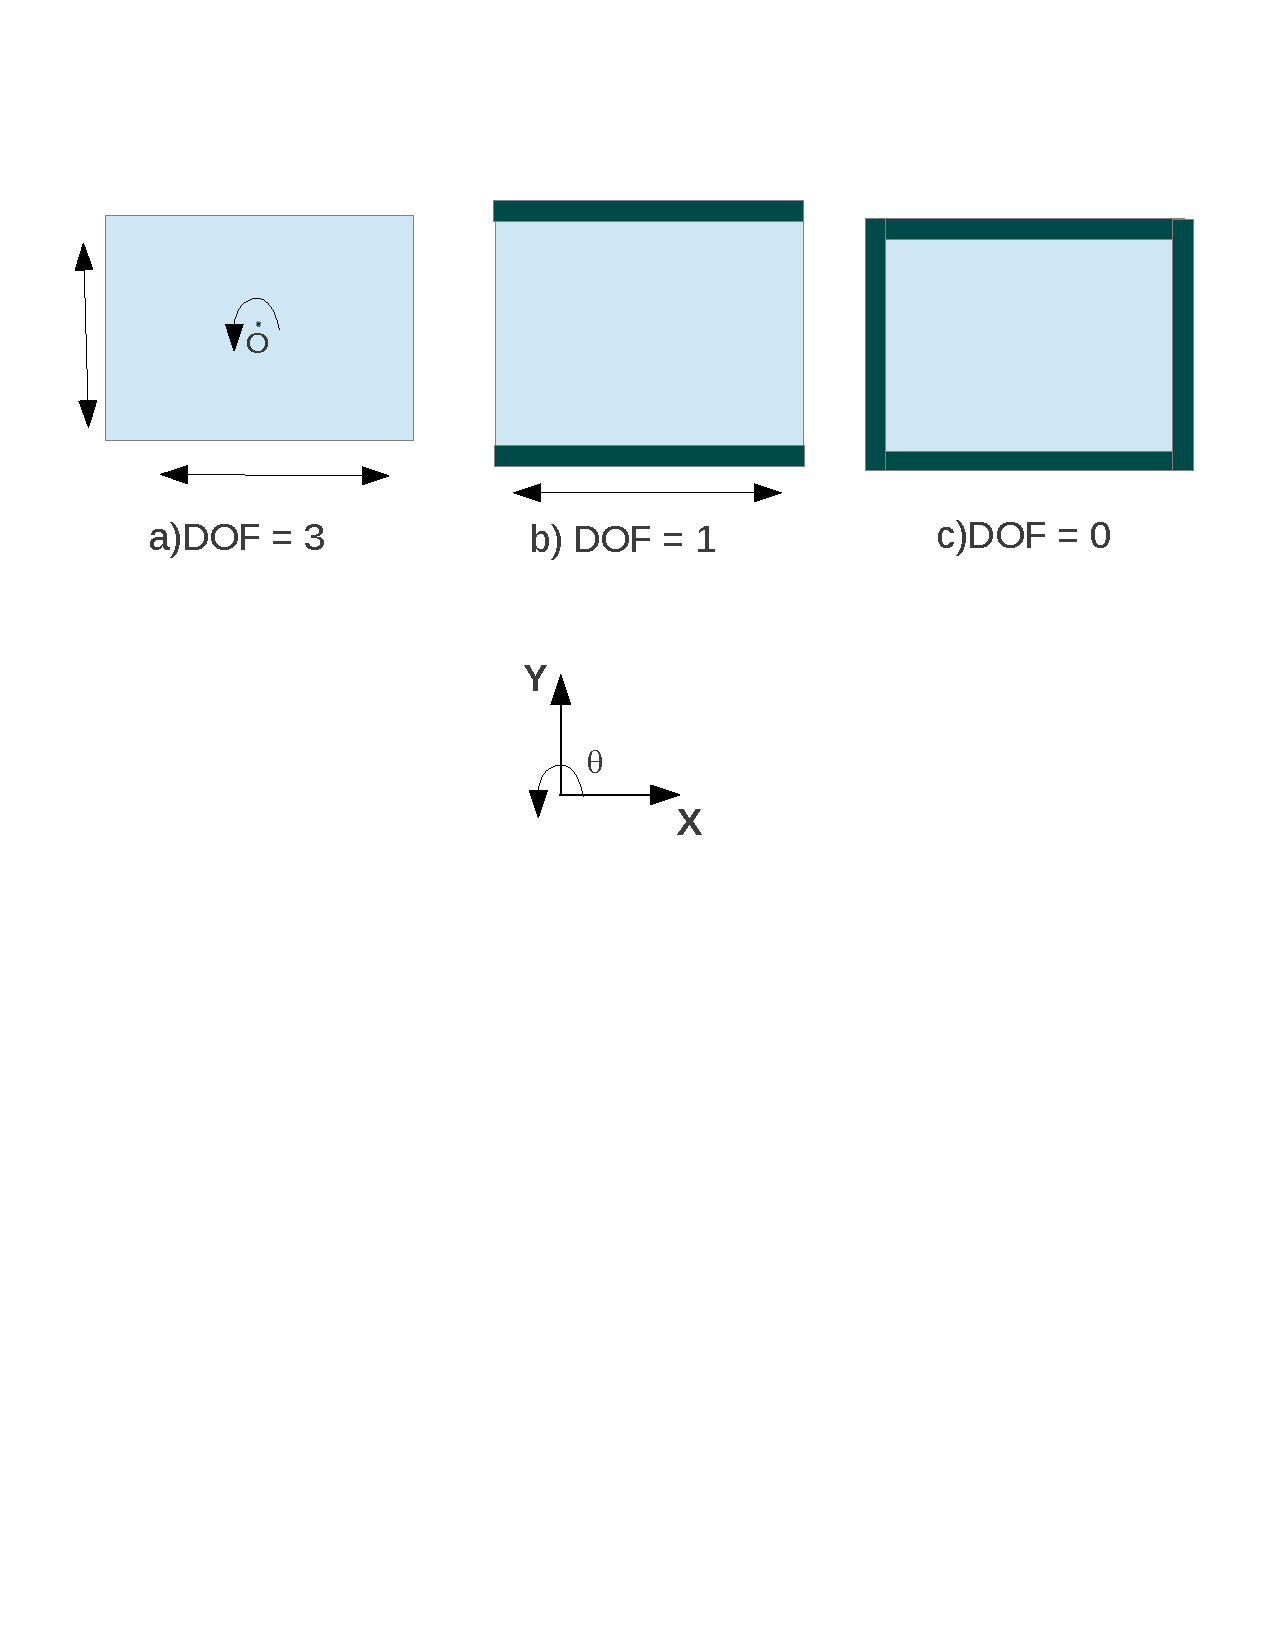
\includegraphics[trim = 0mm 130mm 0mm 20mm, scale = 0.75 ]{Bilder/dof2d.pdf}
    \caption{ Degrees of freedom of two dimensional object}
    \label{fig:dof_2d}
    \end{center}
    \end{figure}
    Figure \ref{fig:dof_2d} show how an object loses its degrees of freedom when it is constrained in 2 dimension space. In Figure \ref{fig:dof_2d} a) represents the unconstrained rectangular object free to move in space, b) represents the rectangular object constrained to move only along x axis and c) represents fully constrained rectangular object. 
    
   The humanoid robots opreates in three dimensional space. When it is freely suspended(it is floating in air) it has six free degrees of freedom. But when it is constrained to its environment, the number of degrees of feedom decreses. In this thesis we aim to estimate the motion of these degrees of freedom of a humanoid robot with respect to a frame of refrence.   
\subparagraph{Illustartion:}    
     \begin{figure}[h]
	    \centering
    	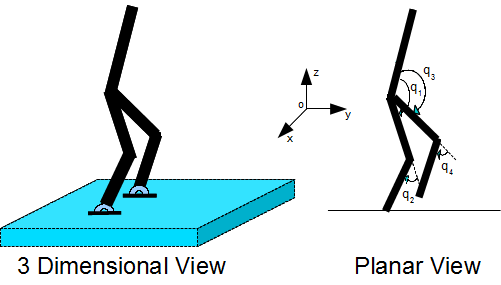
\includegraphics[scale=0.75]{Bilder/robot_flatfloor}
	    \caption{Humanoid robot standing on flat surface}	
	    \label{fig:flat_floor}
    \end{figure}
   Figure \ref{fig:flat_floor} shows a simplified two dimensional version of a humanoid robot standing on the flat surface. The position and orientation of the hip can be determined by computing the forward kinematics of the robot. Forward kinematics is a function of joint angles and it is given as,
    \begin{equation}
    \label{eq:fwkin_flat}
    H_{hip}^s = \text{fwdkin}(q_1,q_2,q_3,q_4),
    \end{equation}
    where $H_{hip}^s$ is the homogeneous transformation matrix position and orientation of the hip with respect to spatial frame. 
    \begin{figure}[h]
	    \centering
    	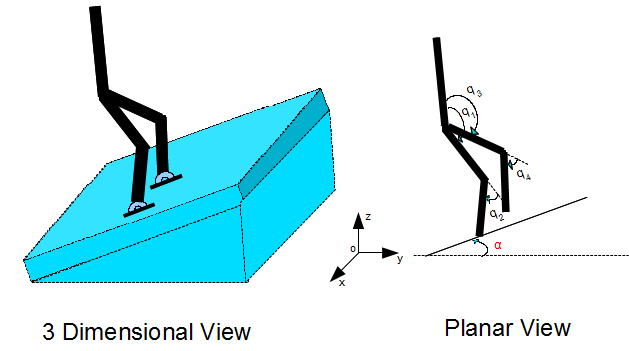
\includegraphics[scale=0.65]{Bilder/robot_slope}
	    \caption{Humanoid robot standing on a slope}	
	    \label{fig:slope}
    \end{figure}
    Figure \ref{fig:slope} shows a humanoid robot staning on the sloping surface. In this case the orientation computed by the forward kinematics function in Equation \ref{eq:fwkin_flat} will be wrong. As we can see in the Figure \ref{fig:slope} there is an additional angle $\alpha$ acting between the surface of the real ground and the slope. There is no direct measuremnt available for this underactuaed degree of freedom. Failure to estimate this angle may lead to  tilting over an edge which might cause the robot to fall on the ground. Estimating this angle will help to achive good balancing in the humanoid robot.

 \section{Methodolgy} 
    Kalman filter is an optimal state estimator for linear systems. The popular nonlinear extensions of Kalman filters used in practice are Extended Kalman filter(EKF) and Unscented Kalman filter(UKF) \citep{oli12}\citep{atk12}\citep{bloe12}. The estimation problem is solved in both versions of Kalman filter. The results are compared based on accuracy of estimates and simulation time. Chapter \ref{ch:st_est} gives brief introduction to state estimation and describes the Kalman filtering algorithm. EKF and UKF algorithms are presented in Chapter \ref{ch:st_est}.

    Two different models used for the purpose of state estimation. They are the multi body system model and the model of Inertial measurement unit(IMU). A multi body system is a modelling foramlism that is used to model the dynamic behaviour of a multi body system. \emph{Toro} is modelled as a multibody system. \emph{Toro} has 25 joints or 25 degrees of freedom. In addition to these 25 degrees of freedom there are 6 underactuad degrees of freedom. Altogether \emph{Toro} has 31 degrees of freedom. State estimation of the multi body system involves estimation of position and velocity of the degrees of freedom of the system. For example in \emph{Toro} has 31 degrees of freedom. The result of estimation problem will be 31 poitions and 31 velocities which leads to 62 states being estimated. Chapter \ref{ch:multi_mdl} deals with the modelling of multibody systems and its implementation in Kalman filtering algorithm. 
    
    A simplified model of IMU is discussed in Chapter \ref{ch:simp_mdl}. State estimation using this model involves estimating the position, orientation, translational velocity, accelerometer bias and gyroscope bias. The position, orientation estimated are the underactuated degrees of freedom and of \emph{Toro}. Translational velocity is the velocity of translationl motion of \emph{Toro}. The number of estimated states are 15. State estimation using this model is more simpler than the multi body system. It is practically implemented on \emph{Toro}.
